\documentclass[a4paper, 11pt]{article}
\usepackage{D:/Documents/latexSettings/myLibrary/raphaelStyle}

%opening
\begin{document}
	
\begin{titlepage}
	
\title{\Huge Motion Control RTFM}
\author{\Large Raphael Rätz}
\maketitle
\end{titlepage}

	



\section{Robot Dynamics}
\subsection{Description of the Dynamics}
\begin{figure}[H]
	\centering
	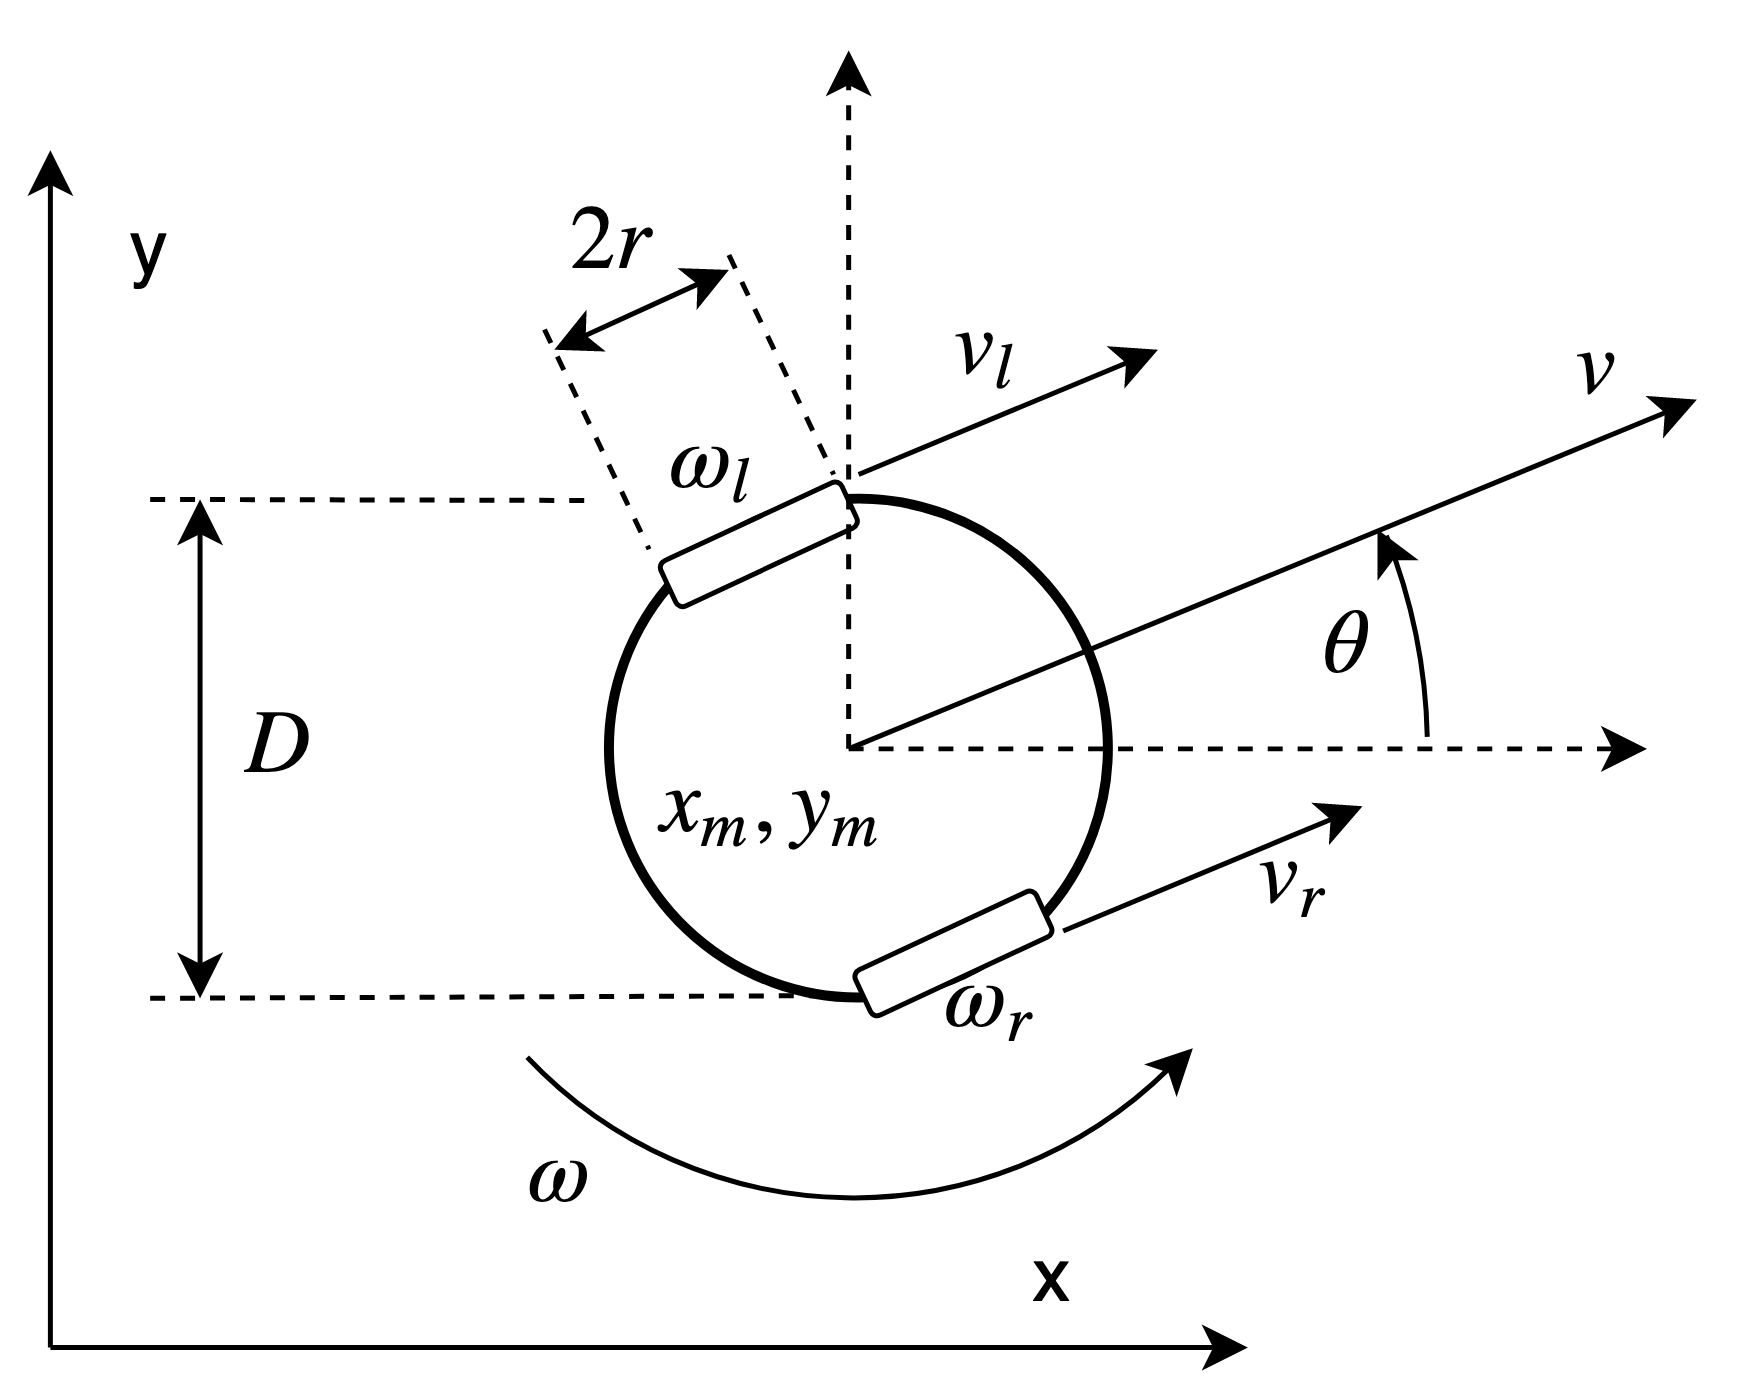
\includegraphics[width=0.7\textwidth]{differentialDriveRobot}
	\caption{Differential drive robot}	
	\label{fig:differentialDriveRobot}	
\end{figure}
\noindent
The subsequent equations describe the dynamics of a differential drive robot. First of all it is important to understand, that a differential drive robot is a non-holonomic robot. There are certain constraints when moving, namely it impossible to move in a transversal direction. The relation of the wheel velocities and the transversal and rotational velocity of a differential drive robot are given by the matrix $T$.
% velocities relation
\begin{equation}
	\begin{bmatrix}
	v\\
	\omega
	\end{bmatrix}
	= T
	\begin{bmatrix}
	\omega_r\\
	\omega_l
	\end{bmatrix}
	\quad with \quad
	T = 
	\begin{bmatrix}
	\frac{r}{2} &\frac{r}{2}\\[4pt] 
	-\frac{r}{D} &\frac{r}{D}
	\end{bmatrix}
\end{equation}
The same relation is valid for the accelerations:
\begin{equation}
\begin{bmatrix}
\dot{v}\\
\dot{\omega}
\end{bmatrix}
= T
\begin{bmatrix}
\dot{\omega}_r\\
\dot{\omega}_l
\end{bmatrix}
\end{equation}
Based on Newtons law of motion, the relation of the transversal force and the torque applied on the robot can be expressed as follows:
% Mass inertia relations
\begin{equation}
\label{inertia mass relations}
	\begin{bmatrix}
	F\\
	\tau
	\end{bmatrix}
	= M
	\begin{bmatrix}
	\dot{v}\\
	\dot{\omega}
	\end{bmatrix}
	\quad with \quad
	M = 
	\begin{bmatrix}
	m &0\\
	0 &J
	\end{bmatrix}
\end{equation}
The translational force in the direction of movement and the torque can as well be expressed as:
% Force torque relations
\begin{equation}
\label{force torque relations}
	\begin{bmatrix}
	F\\
	\tau
	\end{bmatrix}
	= P
	\begin{bmatrix}
	\tau_r\\
	\tau_l
	\end{bmatrix}
	\quad with \quad
	P = 
	\begin{bmatrix}
	\frac{1}{r} &\frac{1}{r}\\[4pt] 
	\frac{D}{2r} &-\frac{D}{2r}
	\end{bmatrix}
\end{equation}
The equations \eqref{force torque relations} and \eqref{inertia mass relations} are equal:
\begin{equation}
P
\begin{bmatrix}
\tau_r\\
\tau_l
\end{bmatrix}
= M
\begin{bmatrix}
\dot{v}\\
\dot{\omega}
\end{bmatrix}
\end{equation}
And finally, the equations of motion without friction can be represented as:
%\begin{equation}
%	\begin{bmatrix}
%	\dot{\omega}_r\\
%	\dot{\omega}_l
%	\end{bmatrix}
%	= \Lambda
%	\begin{bmatrix}
%	\tau_r\\
%	\tau_l
%	\end{bmatrix}
%	\quad with \quad
%	\Lambda = T^{-1}M^{-1}P	
%\end{equation}
%\begin{equation}
%\Lambda =
%\begin{bmatrix}
%\frac{1}{mr^2}+\frac{D^2}{4Jr^2}& \frac{1}{mr^2}-\frac{D^2}{4Jr^2}\\[6pt]
%\frac{1}{mr^2}-\frac{D^2}{4Jr^2}& \frac{1}{mr^2}+\frac{D^2}{4Jr^2}\\[6pt]
%\end{bmatrix}
%\end{equation}

\begin{equation}
\begin{bmatrix}
\dot{v}\\
\dot{\omega}
\end{bmatrix}
= M^{-1}P
\begin{bmatrix}
\tau_r\\
\tau_l
\end{bmatrix}
\end{equation}
By applying the Laplace transform, we obtain the transfer function for the velocity.
\begin{equation}
\begin{bmatrix}
V s\\
\Omega s
\end{bmatrix}
= 
M^{-1}P
\begin{bmatrix}
T_r\\
T_l
\end{bmatrix}
\end{equation}
This can be written in the following form: 
\begin{equation}
\begin{bmatrix}
V\\
\Omega
\end{bmatrix}
= 
\begin{bmatrix}
1/s & 0 \\
0 & 1/s\\
\end{bmatrix}
M^{-1}P
\begin{bmatrix}
T_r\\
T_l
\end{bmatrix}
\end{equation}
At this stage, the motor torque constant $k_t$ and the gear reduction $i_{red}$ can be introduced. The following relationship holds:
\begin{equation}
\begin{bmatrix}
\tau_r\\
\tau_l
\end{bmatrix}
=
\begin{bmatrix}
k_t i_{red} & 0 \\
0 & k_t i_{red}\\
\end{bmatrix}
\begin{bmatrix}
i_r\\
i_l
\end{bmatrix}
\end{equation}
Therefore, 
\begin{equation}
\begin{bmatrix}
V\\
\Omega
\end{bmatrix}
= 
\begin{bmatrix}
1/s & 0 \\
0 & 1/s\\
\end{bmatrix}
M^{-1}P
\begin{bmatrix}
k_t i_{red} & 0 \\
0 & k_t i_{red}\\
\end{bmatrix}
\begin{bmatrix}
I_r\\
I_l
\end{bmatrix}
\end{equation}

in Laplace domain:
\begin{equation}
\begin{bmatrix}
V\\
\Omega
\end{bmatrix}
= 
G(s)
\begin{bmatrix}
I_r\\
I_l
\end{bmatrix}
\quad \textrm{with} \quad
G(s) = 
\begin{bmatrix}
\frac{k_t i_{red}}{m r s} & \frac{k_t i_{red}}{mrs} \\[8pt]
\frac{k_t i_{red}D}{2Jrs} & -\frac{k_t i_{red}D}{2Jrs}\\
\end{bmatrix}
\end{equation}
The system is clearly a couple MIMO system.
\begin{equation}
\begin{split}
	V &= g_{11}(s) I_r + g_{12}(s) I_l \\	
	\Omega &= g_{21}(s) I_r + g_{22}(s) I_l
	\end{split}
\end{equation}

\subsection{Decoupling of the dynamics}
A decoupled system could for example look as follows. It still represents a first order physical system with an inertia/mass, a motor constant and a gear ratio:
\begin{equation}
\begin{bmatrix}
V\\
\Omega
\end{bmatrix}
= 
\begin{bmatrix}
\frac{k_t i}{m s} & 0\\[8pt]
0 &\frac{k_t i}{J s}\\
\end{bmatrix}
\begin{bmatrix}
I_v\\
I_{\omega}
\end{bmatrix}
= G_d(s)
\begin{bmatrix}
I_v\\
I_{\omega}
\end{bmatrix}
\end{equation}
In order to achieve that we need to transform the system input:
\begin{equation}
\begin{bmatrix}
I_r\\
I_l
\end{bmatrix}
= G^{-1}G_d 
\begin{bmatrix}
I_v\\
I_{\omega}
\end{bmatrix}
\end{equation}
As a proof:
\begin{equation}
\begin{bmatrix}
V \\
\Omega
\end{bmatrix}
= G G^{-1}G_d  = G_d
\begin{bmatrix}
I_v\\
I_{\omega}
\end{bmatrix}
\end{equation}

\subsection{Reflected inertia}
\begin{equation}
	\tau_m = \ddot{\theta}_m(J_m + \frac{1}{n^2}J_l)
\end{equation}

\subsection{Equations of motion}
The vector of generalized coordinates $q$ is used:
\begin{equation}
	q = 
	\begin{bmatrix}
	x\\ y\\ \theta\\ \theta_{w,l} \\ \theta_{w,r}\\ \theta_{m,l} \\ \theta_{m,r}
	\end{bmatrix}
\end{equation}
The kinetic energy $KE$ of the system can be described as follows, whereby $J$ is the total robot inertia, $m$ the total mass and $J_m$ the inertia of a motor. The kinetic energy of the wheels are neglected.
\begin{equation}
	KE = \frac{1}{2}m\dot{x}^2 + \frac{1}{2}m\dot{y}^2 + \frac{1}{2}J\dot{\theta}^2 +\frac{1}{2}J_m\dot{\theta}_{m,l}^2 + \frac{1}{2}J_m\dot{\theta}_{m,r}^2
\end{equation}
The following simplification can be made:
\begin{equation}
	\dot{x}^2 + \dot{y}^2 = v^2 \quad \textrm{and} \quad \dot{\theta} = \omega
\end{equation}
This leads to:
\begin{equation}
KE = \frac{1}{2}mv^2 + \frac{1}{2}J\omega^2 +\frac{1}{2}J_m\dot{\theta}_{m,l}^2 + \frac{1}{2}J_m\dot{\theta}_{m,r}^2
\end{equation}
The following relation holds:
\begin{equation}
\begin{bmatrix}
v\\
\omega
\end{bmatrix}
= T
\begin{bmatrix}
\dot{\theta}_{w,l}\\
\dot{\theta}_{w,r}
\end{bmatrix}
\quad with \quad
T = 
\begin{bmatrix}
\frac{r}{2} &\frac{r}{2}\\[4pt] 
-\frac{r}{D} &\frac{r}{D}
\end{bmatrix}
\label{eq:T}
\end{equation}
Also, the angles $\theta_{w,l}$ and $\theta_{w,r}$ are related to the motor angles $\theta_{m,l}$ and $\theta_{m,r}$ by the gear ratio $i$:
\begin{equation}
\begin{bmatrix}
\theta_{w,l} \\ \theta_{w,r}
\end{bmatrix}
= n
\begin{bmatrix}
\theta_{m,l} \\ \theta_{m,r}
\end{bmatrix}
\label{eq:gearRatio}
\end{equation}
The kinetic energy can therefore be rewritten as a function of only $\theta_{m,l}$ and $\theta_{m,r}$:
\begin{equation}
	KE = \frac{1}{2}m\left(   \frac{ir}{2}\dot{\theta}_{m,l} + \frac{nr}{2}\dot{\theta}_{m,r}  \right)^2 +
	\frac{1}{2}J\left(   -\frac{ir}{D}\dot{\theta}_{m,l} + \frac{nr}{D}\dot{\theta}_{m,r}  \right)^2 + 	
	\frac{1}{2}J_m\dot{\theta}_{m,l}^2 + \frac{1}{2}J_m\dot{\theta}_{m,r}^2
\end{equation}
Regrouping leads to:
\begin{equation}
\begin{split}
	KE = &\frac{1}{2}\left(  J_m + \frac{n^2r^2}{4}m + \frac{n^2r^2}{D^2}J \right) \dot{\theta}_{m,l}^2 \\[8pt]
	&\frac{1}{2}\left(  J_m + \frac{n^2r^2}{4}m + \frac{n^2r^2}{D^2}J \right) \dot{\theta}_{m,r}^2 + \\[8pt]
	&\left( \frac{n^2r^2}{4}m - \frac{n^2r^2}{D^2}J   \right)\dot{\theta}_{m,l}\dot{\theta}_{m,r}
\end{split}
\end{equation}
The Lagrangian $L$ can be formed as follows:
\begin{equation}
	L = KE - PE
\end{equation}
Since there is no potential energy involved in this system, $PE = 0$ and therefore $L = KE$. The Lagrange equation states that:
\begin{equation}
	\frac{d}{dt}\left(  \frac{\partial L}{\partial \dot{q}_i} \right) - \frac{\partial L}{\partial q_i} = \tau_i
\end{equation} 
By evaluating this equation for $\theta_{m,l}$ and $\theta_{m,r}$, the motor torques can be found:
\begin{equation}
	\tau_{m,l} = \left(  J_m + \frac{n^2r^2}{4}m + \frac{n^2r^2}{D^2}J \right) \ddot{\theta}_{m,l} + \left( \frac{n^2r^2}{4}m - \frac{n^2r^2}{D^2}J   \right)\ddot{\theta}_{m,r}
\end{equation}
\begin{equation}
\tau_{m,r} = \left(  J_m + \frac{n^2r^2}{4}m + \frac{n^2r^2}{D^2}J \right) \ddot{\theta}_{m,r} + \left( \frac{n^2r^2}{4}m - \frac{n^2r^2}{D^2}J   \right)\ddot{\theta}_{m,l}
\end{equation}
And in matrix notation:
\begin{equation}
	\begin{bmatrix}
	\tau_{m,l}\\ \tau_{m,r}
	\end{bmatrix}
	= 
	M
	\begin{bmatrix}
	\ddot{\theta}_{m,l}\\ \ddot{\theta}_{m,r}
	\end{bmatrix}
	\quad \textrm{with} \quad 
	M = 
	\begin{bmatrix}
	J_m + \frac{n^2r^2}{4}m + \frac{n^2r^2}{D^2}J & \frac{n^2r^2}{4}m - \frac{n^2r^2}{D^2}J\\[8pt]
	\frac{n^2r^2}{4}m - \frac{n^2r^2}{D^2}J & J_m + \frac{n^2r^2}{4}m + \frac{n^2r^2}{D^2}J\\
	\end{bmatrix}
\end{equation}
With the above equation, the equation of motion has been found. Using equations \eqref{eq:T} and \eqref{eq:gearRatio}, the equation can be transformed into:
\begin{equation}
	\begin{bmatrix}
	\tau_{m,l}\\ \tau_{m,r}
	\end{bmatrix}
	= 
	\frac{1}{n}MT^{-1}
	\begin{bmatrix}
	\dot{v}\\ \dot{\omega}
	\end{bmatrix}
\end{equation}
Or, the translational and angular acceleration of the robot can be expressed as a function of the motor torques:
\begin{equation}
\begin{bmatrix}
\dot{v}\\ \dot{\omega}
\end{bmatrix}
= 
nTM^{-1}
\begin{bmatrix}
\tau_{m,l}\\ \tau_{m,r}
\end{bmatrix}
\end{equation}
Then, the torque constant $k_t$ which describes the motor torque in function of the motor current can be introduced:
\begin{equation}
\begin{bmatrix}
\tau_{m,l} \\ \tau_{m,r}
\end{bmatrix}
= k_t
\begin{bmatrix}
i_{m,l} \\ i_{m,r}
\end{bmatrix}
\label{eq:kt}
\end{equation}
This leads to:
\begin{equation}
\begin{bmatrix}
\dot{v}\\ \dot{\omega}
\end{bmatrix}
= 
k_tnTM^{-1}
\begin{bmatrix}
i_{m,l}\\ i_{m,r}
\end{bmatrix}
\end{equation}
At this point, the equations of motion can be transformed into the Laplace domain, $s$ being the Laplace operator:
\begin{equation}
\begin{bmatrix}
Vs\\ \Omega s
\end{bmatrix}
= 
k_tnTM^{-1}
\begin{bmatrix}
I_{m,l}\\ I_{m,r}
\end{bmatrix}
\end{equation}
And therefore, the velocities can be expressed as follows, with $G(s)$ being the transfer function describing the system behaviour in terms of velocity due to current inputs on the motors:
\begin{equation}
\begin{bmatrix}
V\\ \Omega
\end{bmatrix}
= G(s)
\begin{bmatrix}
I_{m,l}\\ I_{m,r}
\end{bmatrix}
\quad \textrm{with} \quad
G(s) = k_tnTM^{-1}\frac{1}{s} 
\end{equation}
Let's have a closer look at $G(s)$:
\begin{equation}
	G(s) = 
	\begin{bmatrix}
	g_{11} & g_{12} \\
	g_{21} & g_{22}
	\end{bmatrix}
	=
	\begin{bmatrix}
	\frac{k_tnr}{(mn^2r^2 + 2J_m)s} & \frac{k_tnr}{(mn^2r^2 + 2J_m)s}\\[8pt]
	-\frac{k_tnrD}{(J_mD^2 + 2Jn^2r^2)s} & \frac{k_tnrD}{(J_mD^2 + 2Jn^2r^2)s}
	\end{bmatrix}
\end{equation}
As expected, the system is coupled. For example, an input torque on the left motor provokes a translational and an angular velocity change. The same is of course valid for the right motor. In control theory, such a system is called a coupled MIMO (mulitple input, multiple output) system. It would be favourable to have a decoupled system, where the change of one system output is the result of only one system input. The coupling would be eliminated if 
\begin{equation}
	G_d(s) = 
	\begin{bmatrix}
	g_{11} & 0 \\
	0 & g_{22}
	\end{bmatrix}
\end{equation}
The system behaviour $G(s)$ itself cannot be changed, but it is possible to transform the input such that the system behaves like $G_d(s)$. So let's suppose that the input (in this case the motor currents) are a function of a decoupled input $[I_{trans}, I_{rot}]^T$ such that:
\begin{equation}
	\begin{bmatrix}
	I_{m,l} \\ I_{m,r}
	\end{bmatrix}
	= H(s)
	\begin{bmatrix}
	I_{trans} \\ I_{rot}
	\end{bmatrix}
	\label{eq:inputTrans}
\end{equation}
This means that:
\begin{equation}
	\begin{bmatrix}
	V\\ \Omega
	\end{bmatrix}
	= G(s)H(s)
	\begin{bmatrix}
	I_{trans}\\ I_{rot}
	\end{bmatrix}
	= G_d(s)
	\begin{bmatrix}
	I_{trans}\\ I_{rot}
	\end{bmatrix}
\end{equation}
Consequently, the system can be decoupled with a surprisingly simple input transformation:
\begin{equation}
	H(s) = G^{-1}(s)G_d(s) = 
	\begin{bmatrix}
	\frac{1}{2} & -\frac{1}{2}\\[6pt]
	\frac{1}{2} & \frac{1}{2}
	\end{bmatrix}
\end{equation}
This means that by applying this input transformation \eqref{eq:inputTrans}, the robot behaves like two decoupled systems. Therefore, two independent controllers can be designed.
\begin{equation}
	V = g{11}(s)I_{trans} \quad \textrm{and} \quad \Omega = g{22}(s)I_{rot}
\end{equation}

% --------------------------------------------------------------------------------------------------




\newpage
\section{Velocity control}
An ADRC type controller is chosen for the two independent velocity controls. The basic idea of ADRC is to understand a system as follows:
\begin{equation}
	\ddot{y} = \dot{v} = f(y,\dot{y}, f_{ext}, t) + bu
\end{equation}


\newpage
%\section{Code Composer}
%\begin{itemize}
%	\item righ click on project$\rightarrow$Properties$\rightarrow$CSS General$\rightarrow$ Configuration: F2837x-FLASH
%\end{itemize}
%
%\section{Hardware}
%\subsection{Getting Started}
%\begin{itemize}
%	\item J1, J2, J3 should be removed
%	\item The debug probe connects only if the device is in the emulation boot mode (TRST switch in the UP-1 position) 
%	\item All switches of S1 are on
%	\item The S4 switch should be OFF in order to allow for the nFAULT pin from the DRV8305 to report. (does not exist on delfino...)
%\end{itemize}
%\subsection{H-bridge}
%\begin{itemize}
%	\item ALWAYS either PwmARegs.CMPA.bit.CMPA = 0 or PwmBRegs.CMPA.bit.CMPA = 0 !!!
%	\item When using Ta and Tb: Ta = -1 $\rightarrow$ PwmARegs.CMPA.bit.CMPA = 0 and Ta = 1 $\rightarrow$ PwmARegs.CMPA.bit.CMPA = max !!!
%	\item Pay attention to undervoltage on VDD. Default value is 
%	\item http://modularcircuits.tantosonline.com/blog/articles/h-bridge-secrets/asynchronous-sign-magnitude-drive/
%	\item shunt A goes to to Adc_in_C2 (input 2 block C) of the Delfino
%	\item AdccResultRegs.ADCPPB1RESULT should be current A	
%	\item $\rightarrow$ AdccRegs.ADCPPB1CONFIG.CONFIG = 2 (connects block adc 2 with the post processing block PBB)
%	\item shunt B goes to Adc_in_B2
%	\item shunts are note directly connected!!! via ampli op!
%\end{itemize}

%\begin{equation}
%t_{opt} = -\frac{L\,\ln\left(\frac{R\,\left({\mathrm{e}}^{-\frac{2\,R\,T_{1}}{L}}+{\mathrm{e}}^{-\frac{R\,T_{2}}{L}}-{\mathrm{e}}^{-\frac{R\,\left(T_{1}+T_{2}\right)}{L}}+1\right)}{L\,T_{2}}+1\right)}{R}
%\end{equation}
%????

\newpage
\section{Kinematic Position Controller}
\subsection{Kinematics}
\begin{figure}[H]
	\centering
	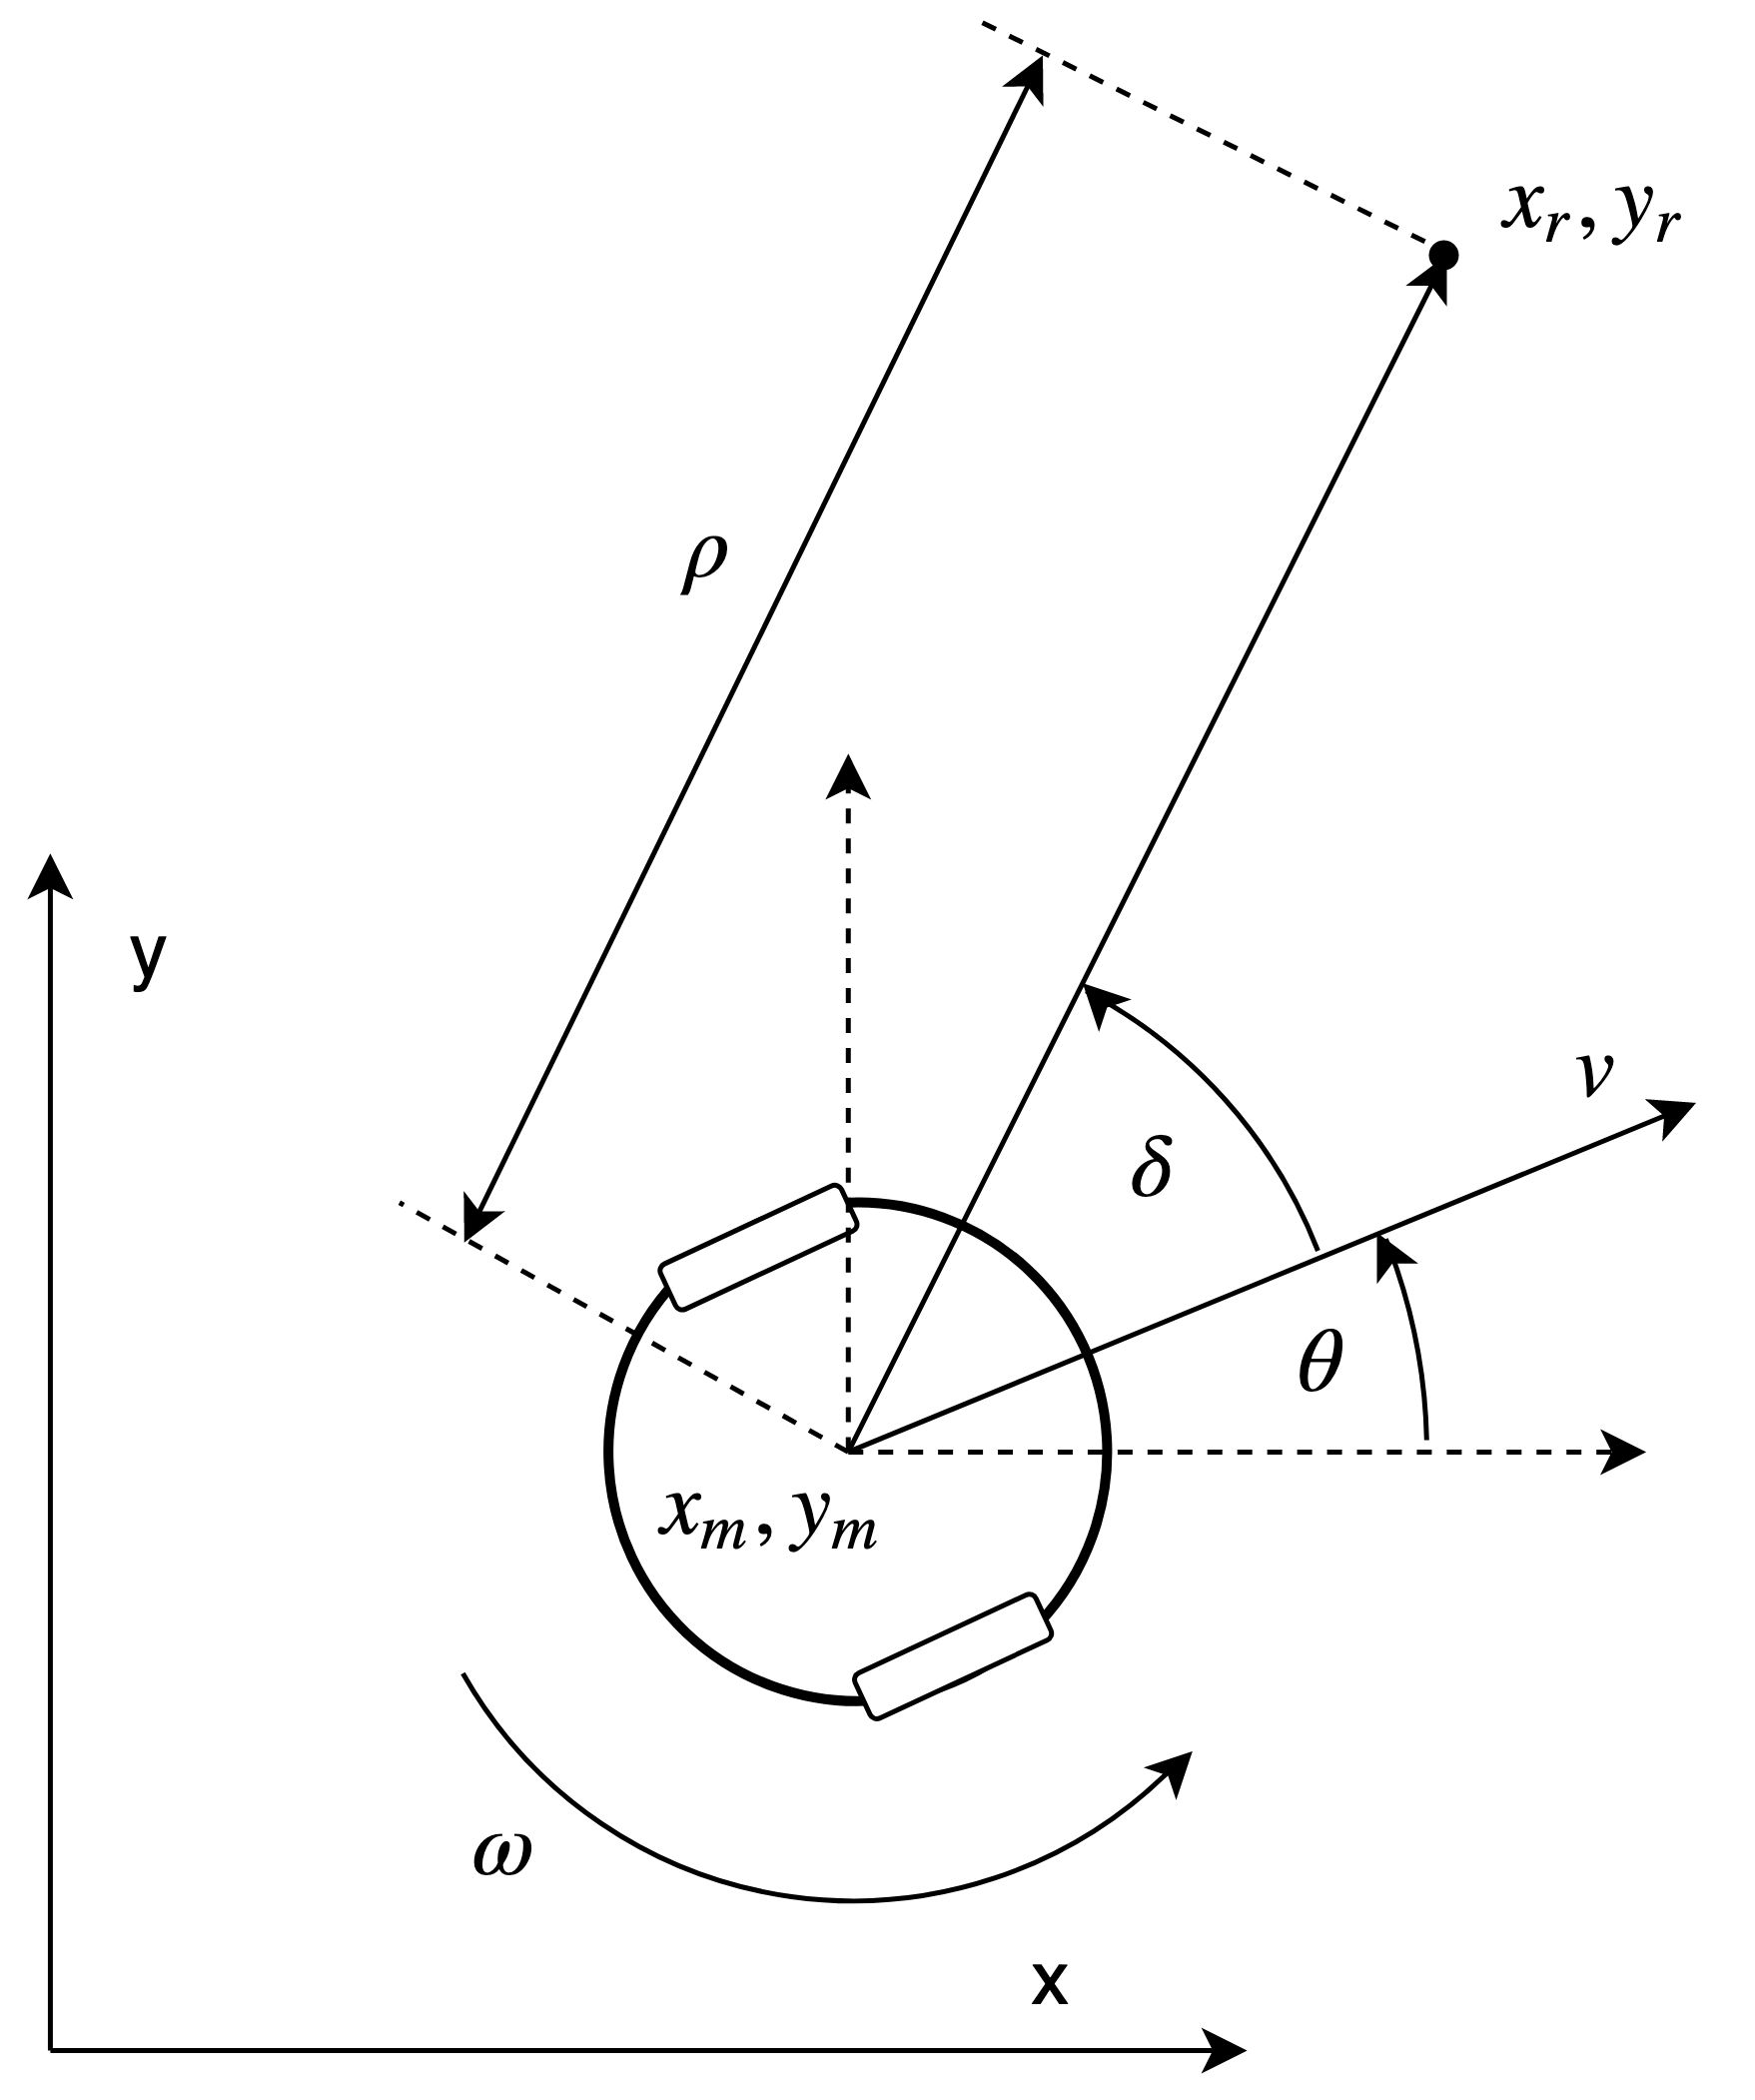
\includegraphics[width=0.8\textwidth]{robotPosition}
	\caption{Robot pose and goal position $x_r$, $y_r$}	
	\label{fig:robotPosition}	
\end{figure}
\noindent
Figure \ref{fig:robotPosition} shows the measured pose of the robot $(x_m, y_m, \theta)$ as well as the goal position ($x_r,y_r$). The angle $\theta$ is measured with respect to the global x-axis. The robot moves with a translational velocity $v$ and an angular velocity $\omega$. The non-holonomic behaviour of the differential drive robot can be represented as follows:
\begin{equation}
\begin{bmatrix}
\dot{x}\\
\dot{y}\\
\dot{\theta}
\end{bmatrix}
=
\begin{bmatrix}
cos(\theta)	&0\\
sin(\theta)	&0\\
0			&1\\
\end{bmatrix}
\begin{bmatrix}
v\\
\omega
\end{bmatrix}
\end{equation}
The Euklidian distance from the robots position ($x_m, y_m$) to the reference position ($x_r, y_r$) is denoted $\rho$. The angle $\delta$ describes the difference between the momentary heading of the robot and the heading of the goal position. 
Rhe distance $\rho$ can be calculated as:
\begin{equation}
	\rho = \sqrt{(x_r-x_m)^2 + (y_r-y_m)^2}
\end{equation}
And the angle $\delta$ as follows:
\begin{equation}
\delta = atan2(y_r-y_m, x_r-x_m) - \theta
\end{equation}
Next, let's take the derivative of $\rho$ and $\delta$. First, using the chain rule and trigonometric identities, $\dot{\rho}$ is computed as:
\begin{equation}
\begin{aligned}
	\dot{\rho} 
	&= \frac{-(x_r - x_m)\dot{x}_m - (y_r - y_m)\dot{y}_m}{\sqrt{(x_r - x_m)^2 + (y_r - y_m)^2} }\\
	&= -\frac{(x_r - x_m)}{\rho} \dot{x}_m - \frac{(y_r - y_m)}{\rho}\dot{y}_m\\
	&= -\cos(\delta + \theta) \cos(\theta)v - \sin(\delta + \theta) \sin(\theta)v\\
	&= -\cos(\delta) v\\
\end{aligned}
\end{equation}

Hence, the dynamics of $\rho$ and $\delta$ can be written as:
\begin{equation}
\begin{bmatrix}
\dot{\rho}\\[6pt]
\dot{\delta}
\end{bmatrix}
= 
\begin{bmatrix}
-vcos(\delta)\\[6pt]
\frac{v}{r}sin(\delta) - \omega
\end{bmatrix}
\end{equation}


\subsection{Lyapunov based Controller}
A function $V$ is called a Lyapunov function candidate if it satisfies the requirements: 
\begin{itemize}
	\item $V(x) = 0$ if and only if $x = 0$
	\item $V(x) > 0$ if and only if $x \not=0$
	\item $\dot{V}(x) \le 0$ for all values $x \not = 0$ 
\end{itemize}
The following Lyapunov function candidate with two states $x_1$ and $x_2$ has been chosen in this case. 
\begin{equation}
V(x) = \frac{1}{2}x^Tx = \frac{1}{2}x_1^2 + \frac{1}{2}x_2^2
\end{equation}
A dynamic system is said to be globally asymptotically stable if it can be shown that $\dot{V}(x) < 0$ for $x \not = 0$. The corresponding derivative of the chosen $V(x)$ is:
\begin{equation}
\dot{V}(x) = x_1\dot{x}_1 + x_2\dot{x}_2
\end{equation}
When setting $x_1 = \rho$ and $x_2 = \delta$, the derivative of $V$ takes the following form:
\begin{equation}
\dot{V} = -v \rho cos(\delta) + \delta (\frac{v}{\rho} sin(\delta) - \omega)
\end{equation}
The left part of this equation can be forced to be negative by defining the translational velocity control law:
\begin{equation}
	v = K_{\rho} cos(\delta) \rho \qquad \textrm{with} \quad K_{\rho} > 0
	\label{eq:vel}
\end{equation}
The right term of $\dot{V}$ becomes therefore:
\begin{equation}
	\delta (\frac{K_{\rho} cos(\delta) \rho}{\rho} sin(\delta) - \omega) = \delta\left( K_{\rho}cos(\delta) sin(\delta) - \omega \right)
\end{equation}
In order to force the total expression of $\dot{V}$ to be negative, a simple proposition is made. The right term can be forced to be zero by defining the angular velocity as:
\begin{equation}
	\omega = K_{\rho} sin(\delta) cos(\delta)
	\label{eq:omega}
\end{equation}
Consequently, the total expression of $\dot{V}$ becomes as follows, which is negative for if $x \not = 0$ and zero if $x = 0$.
\begin{equation}
\dot{V} = -K_{\rho} cos(\delta)^2 \rho^2 \le 0 
\end{equation}
%\qquad \textrm{for} \quad \rho \not = 0
According to Lyapunov, the robot is therefore asymptotically stable if using the control laws \eqref{eq:vel} and \eqref{eq:omega} because the derivative of $V$ is globally negative except from the origin where it is zero. The two control laws necessitate only one tuning parameter $K_{\rho}$, which makes this controller easily tunable despite its non-linear nature. 

\subsection{Practical consideration: damping around origin}
Due to the non-holonomic nature of the differential robot, the robot may start rotating strongly around the origin ($x_m \approx x_r$ and $y_m \approx y_r$) in order to converge. Imagine that the robot arrives a few tenth of a millimetre laterally to the goal position. Its only possibility to correct would be to turn at its momentary position and move slightly forward or backwards. If the position is still not perfect, it will continue until it arrives at a position where the error is too small in comparison the the mechanical frictions in the system. Especially the command of $\omega$ it is unwanted to be unstable or sensitive to external perturbations. It is very undesired that the robot starts rotating around the origin. It is therefore proposed to dampen or weaken the control law of the angular velocity around the origin. The following function $g(\rho)$ is proposed \footnote{In the code, "alphaSquared" might be used instead of "alpha". However, "alphaSquared = $\alpha$"}:
\begin{equation}
g(\rho) = \left(1- \frac{\alpha}{\rho^2 +\alpha}\right)
\end{equation}
The characteristic of this function is that its value is approximately 1 for $\rho^2 \gg \alpha $ which guarantees proper functioning of the Lyapunov based control law. However as $\rho$ approaches zero, $g(\rho)$ decreases smoothly to zero.
%The value $\alpha$ allows to adjust the moment when the function will decelerate. A new parameter $b$ is introduced. The value $v_0b$ is the desired function value at the point $r = r_b$. The velocity function can be adjusted by using the following equation. If for example a velocity of $v=0.8v_0$ is desired at a distance of $r = 4$, the parameter $\alpha$ would be equal to $2$.
%\begin{equation}
%\alpha = \sqrt{\frac{1-b}{b}}r_b
%\end{equation}
\begin{figure}[H]
	\centering
	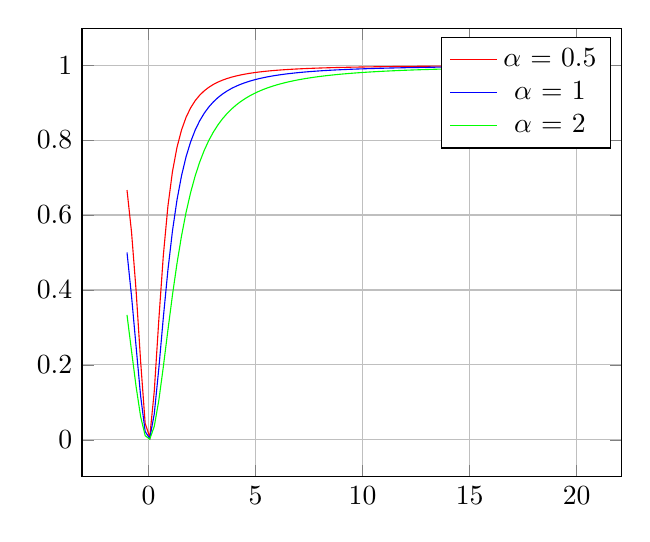
\begin{tikzpicture}
	\begin{axis}[grid=both]
	\addplot[domain=-1:20, samples=100, color=red]{1- 0.5/(x^2 +0.5)};
	\addlegendentry{$\alpha$ = 0.5}
	\addplot[domain=-1:20, samples=100, color=blue]{1- 1/(x^2 +1)};
	\addlegendentry{$\alpha$ = 1}
	\addplot[domain=-1:20, samples=100, color=green]{1- 2/(x^2 +2)};
	\addlegendentry{$\alpha$ = 2}
	\end{axis}
	\end{tikzpicture}
\end{figure}
\noindent
The function $g(\rho)$ is multiplied with the control law for the angular velocity $\omega$. The final control laws are therefore given by equation \eqref{eq:omegaFinal} and \eqref{eq:velFinal}. Proximate to the origin, the control law for $\omega$ is almost zero, which avoids undesired rotations.
\begin{equation}
\boxed{v= K_{\rho} cos(\delta) \rho}
\label{eq:velFinal}	
\end{equation} 
\begin{equation}
	\boxed{\omega = K_{\rho} g(\rho) sin(\delta) cos(\delta)}
	\label{eq:omegaFinal}	
\end{equation}


\section{Motion Planning}
\subsection{Trapezoidal Motion Planner}
In order to guarantee a smooth trajectory, a trapezoidal motion planner is used. It provides trajectories with finite acceleration and deceleration. A trapezoidal profile as it is shown in figure \ref{fig:trapMotionExample} can be calculated based on the desired acceleration $a_{max}$, the desired velocity $v_{max}$ and the desired distance $\Delta s$. The acceleration, the velocity and the covered distance at a given time $t$ are given by the set of equations \eqref{avs}. Note that for these equations, $\Delta s$ is considered to be positive.
\begin{figure}[H]
	\centering
	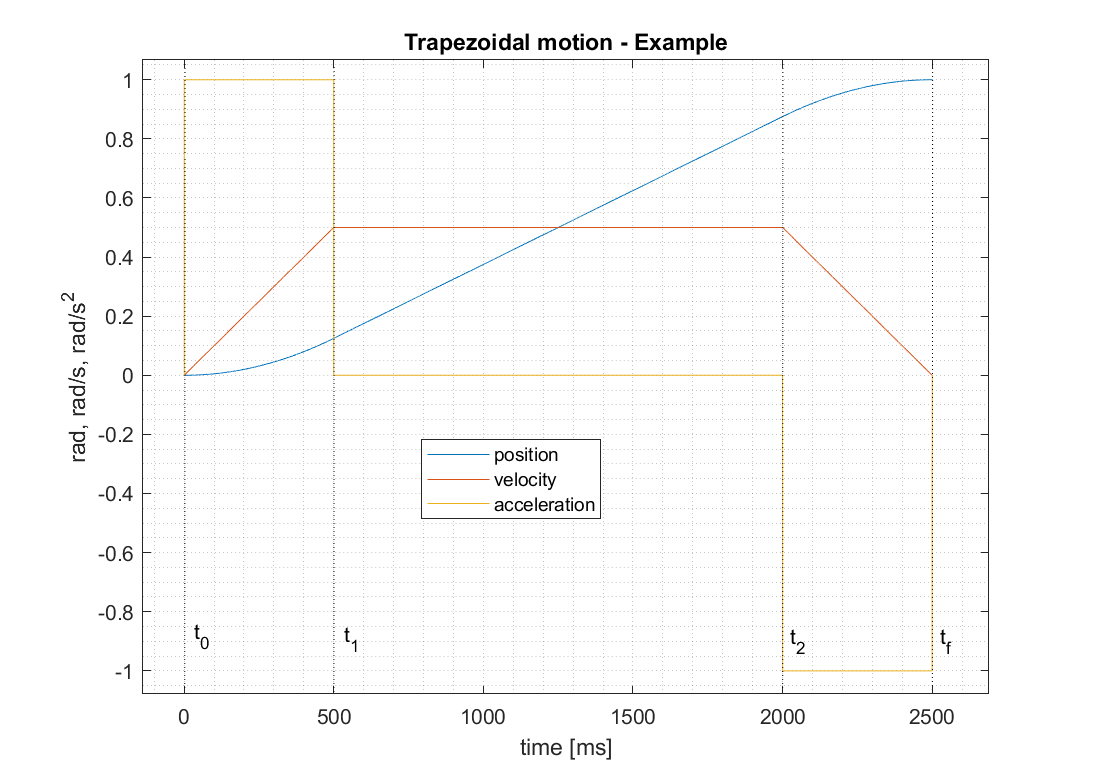
\includegraphics[width=\textwidth]{trapMotionExample}
	\caption{Trapezoidal motion profile}	
	\label{fig:trapMotionExample}	
\end{figure}
\noindent 
\begin{equation}
\label{avs}
\begin{split}
a(t) =
&\begin{cases}
a_{max} \qquad &\textrm{for} \quad t<t_1\\
0 		       &\textrm{for} \quad t_1\leq t<t_2\\
-a_{max} 	   &\textrm{for} \quad t_2 \leq t < t_f\\
\end{cases}\\
v(t) =
&\begin{cases}
a_{max}t \qquad &\textrm{for} \quad t<t_1\\
v_{max} 	      &\textrm{for} \quad t_1\leq t<t_2\\
a_{max}(t_1+t_2-t) 	   &\textrm{for} \quad t_2 \leq t < t_f\\
\end{cases}\\
s(t) =
&\begin{cases}
\frac{1}{2}a_{max}t^2 \qquad &\textrm{for} \quad t<t_1\\
\frac{1}{2}a_{max}t_1^2 + v_{max}(t-t_1)		       &\textrm{for} \quad t_1\leq t<t_2\\
\frac{1}{2}a_{max}t_1^2 + v_{max}(t_2-t_1) + \frac{1}{2}a_{max}(t-t_2)^2	   &\textrm{for} \quad t_2 \leq t < t_f\\
\end{cases}\\
\end{split}
\end{equation}
The corresponding time instants $t_1$, $t_2$ and $t_f$ can be calculated by the equations \eqref{t1t2tf}.

\newpage
\begin{equation}
\label{t1t2tf}
\begin{split}
t_1 =
&\begin{cases}
\sqrt{\frac{\Delta s}{a_{max}}}  \qquad &\textrm{if} \quad \Delta s \leq \frac{v_{max}^2}{a_{max}}\\[10pt]
\frac{v_{max}}{a_{max}}  \qquad &\textrm{otherwise} \\
\end{cases}\\
t_2 =
&\begin{cases}
t_1  \qquad &\textrm{if} \quad \Delta s \leq \frac{v_{max}^2}{a_{max}}\\[10pt]
\frac{\Delta s}{v_{max}}  \qquad &\textrm{otherwise} \\
\end{cases}\\
t_f =
&\begin{cases}
2t_1  \qquad &\textrm{if} \quad \Delta s \leq \frac{v_{max}^2}{a_{max}}\\[10pt]
t_1 + t_2   \qquad &\textrm{otherwise} \\
\end{cases}\\
\end{split}
\end{equation}
If the acceleration $a_0$ is not high enough or if the distance $\Delta s$ is too short, it is possible that the velocity $v_{max}$ can not be reached and therefore $t_1=t_2$. This kind of motion is known as triangular motion profile and is illustrated in figure \ref{fig:triangMotionExample}
\begin{figure}[H]
	\centering
	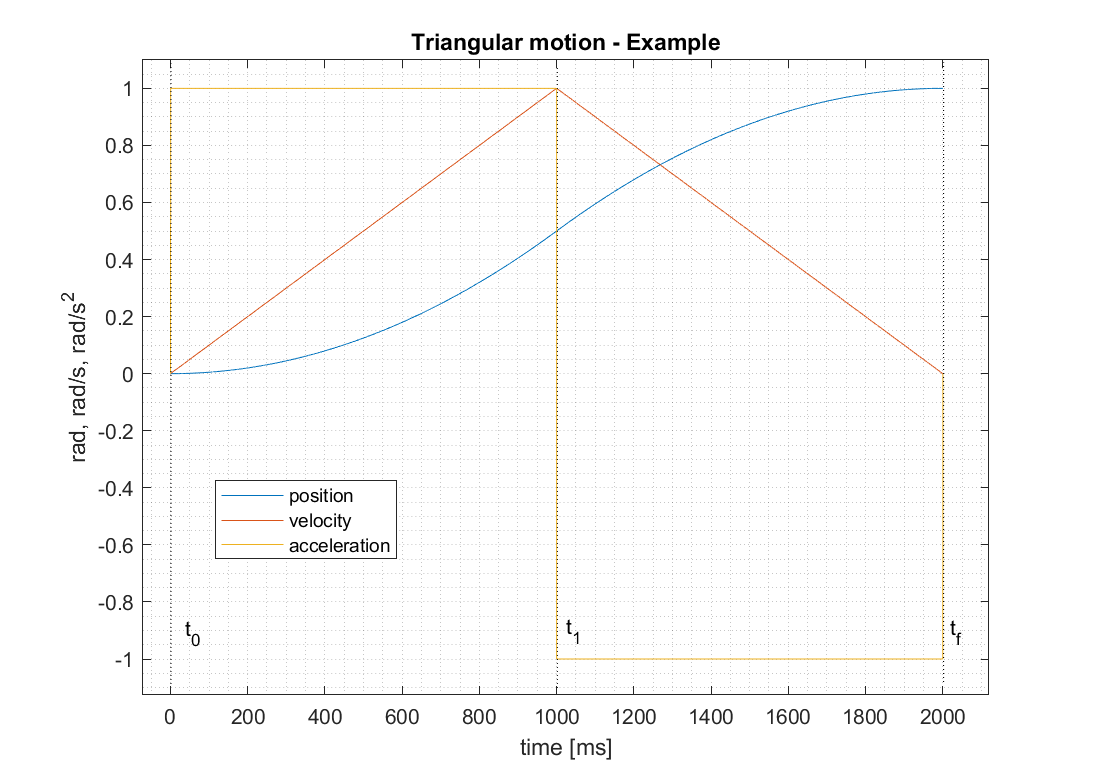
\includegraphics[width=\textwidth]{triangMotionExample}
	\caption{Triangular motion profile}	
	\label{fig:triangMotionExample}	
\end{figure}
\noindent
\subsection{Bezier Curves}
The higher level path planner (Beaglebone) provides a path which consists of several segments of cubic Bezier curves. One cubic Bezier curve is defined as: 
\begin{equation}
\begin{split}
	\mathbf{b}(u) = (1-u)^3\mathbf{p_0} + 3(1-u)^2u\mathbf{p_1} + 3(1-u)u^2\mathbf{p_2} +  u^3\mathbf{p_3}\\[8pt]
	\textrm{with} \quad 
	\mathbf{p_n} = 
	\begin{bmatrix}
	x_n\\ y_n
	\end{bmatrix} \quad \textrm{and} \quad
	0 \le u \le 1 
\end{split}
	\label{eq:bezier}
\end{equation}
This equation can be expanded and rearranged to the form:
\begin{equation}
	\mathbf{b}(u) = (-\mathbf{p_0} + \mathbf{p_1} - \mathbf{p_2} + \mathbf{p_3})u^3 + (3\mathbf{p_0} - 6\mathbf{p_1} + 3\mathbf{p_2})u^2 + (-3\mathbf{p_0} + 3\mathbf{p_1})u + \mathbf{p_0}
\end{equation}
The analytical expression for the length of a Bezier curve is rather complicated and consists of several square roots (always having two solutions). Yet, numerical integration can be used in order to calculate the length. One Bezier curve is divided in $K$ segments. The length of each of these smaller segments is approximated by linear segments. The total length $L$ is simply calculated as sum of the lengths of the linear segments. 
\begin{equation}
	L = \sum_{k = 0}^{K-1} \sqrt{  \left( b_x(u_{k+1}) - b_x(u_k) \right)^2  + \left(b_y(u_{k+1}) - b_y(u_k) \right)^2 } 
	\quad \textrm{with} \quad u_k = \frac{k}{K}
\end{equation}


\newpage
\section{Current Control}
\begin{figure}[H]
	\centering
	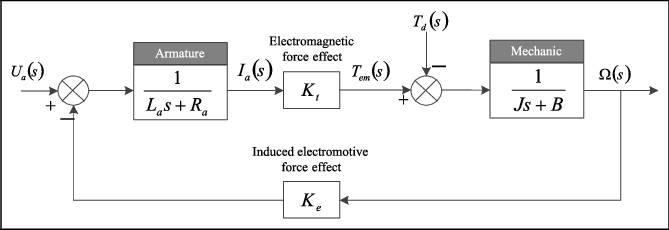
\includegraphics[width=\textwidth]{dcMotorSchema}
	\caption{Block schema of DC motor}		
\end{figure}
In order to simplify things, the inertia $J$ contains not only the rotor inertia, but the total inertia opposing to the motor torque (including robot mass, inertia, etc..). The same is true for the friction term $b$. 

Since the motor torque is proportional to the motor current, we have direct control of the torque by using a current controller. The transfer function $G_{iu}(s)$ which describes the behaviour of the motor current in function of the input voltage in the frequency domain can be represented as follows:
\begin{equation}
G_{iu}(s) =  \frac{J}{K_tK_e}\cdot\frac{s}{\frac{LJ}{K_tK_e}s^2 + \frac{RJ}{K_tK_e}s + 1}
\end{equation}
The dynamic behaviour of the motor current can be simplified to \eqref{RL circuit}.
\begin{equation}
\label{RL circuit}
G_{iu}(s) \approx \frac{1}{Ls + R}
\end{equation}
\begin{figure}[H]
	\centering
	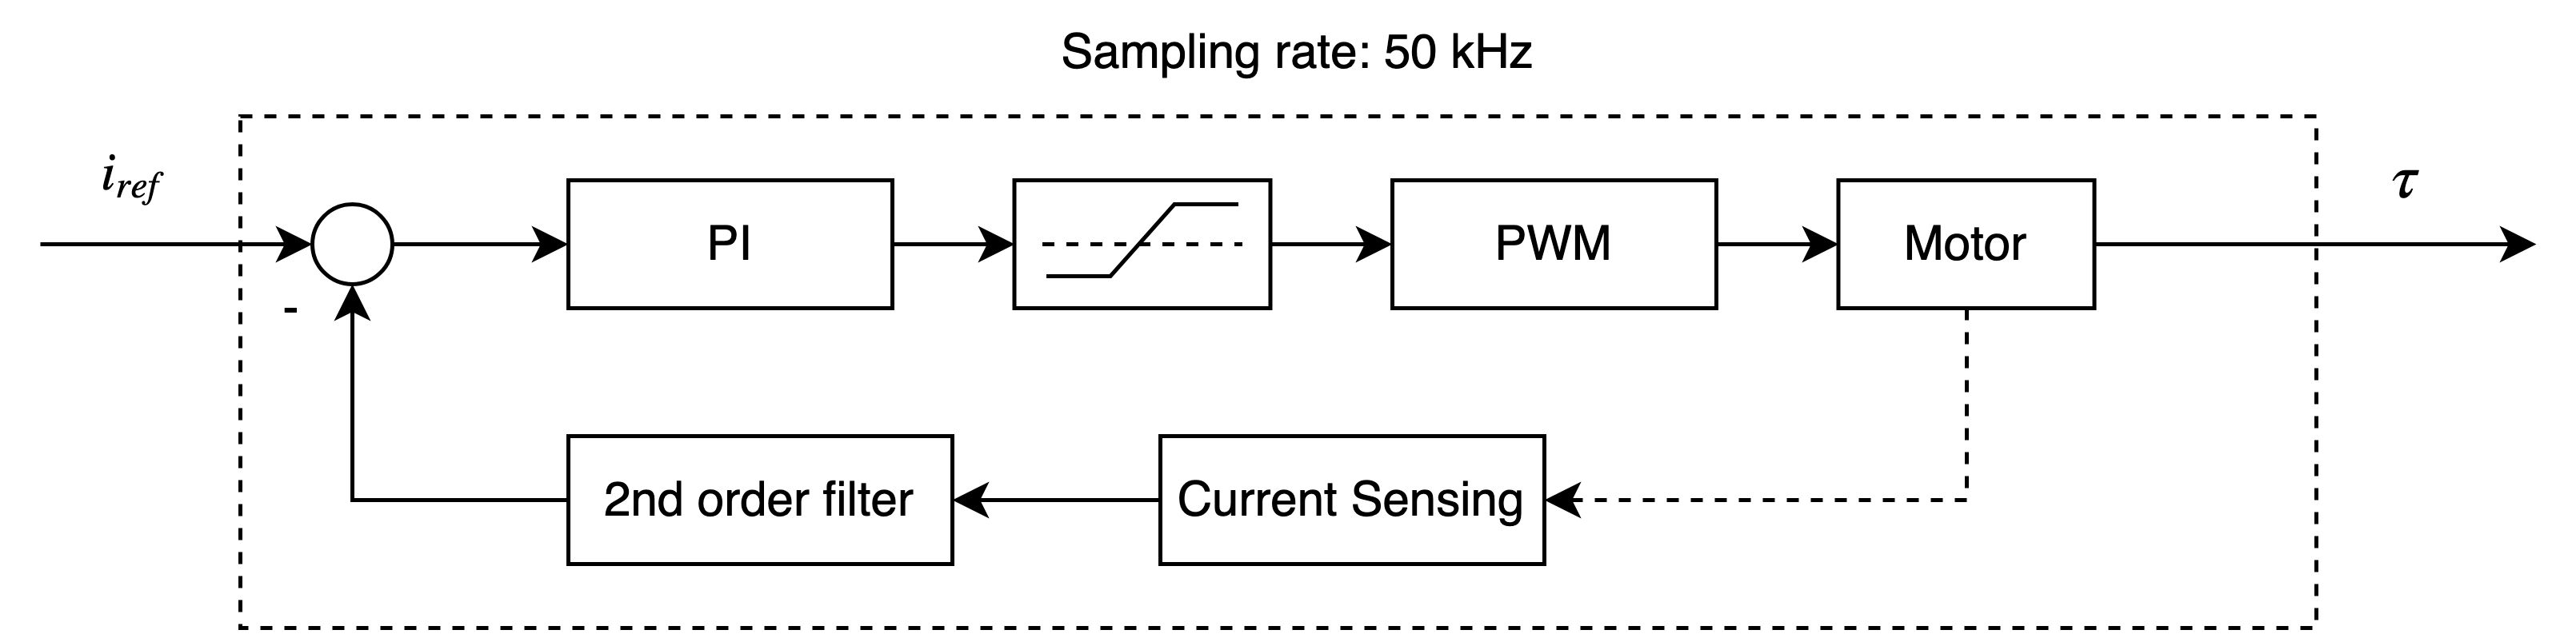
\includegraphics[width=0.8\textwidth]{currentControl}
	\caption{Block schema of the current control}	
	\label{fig:currentControl}	
\end{figure}
\noindent 


\newpage
\section{Velocity Control}
\begin{figure}[H]
	\centering
	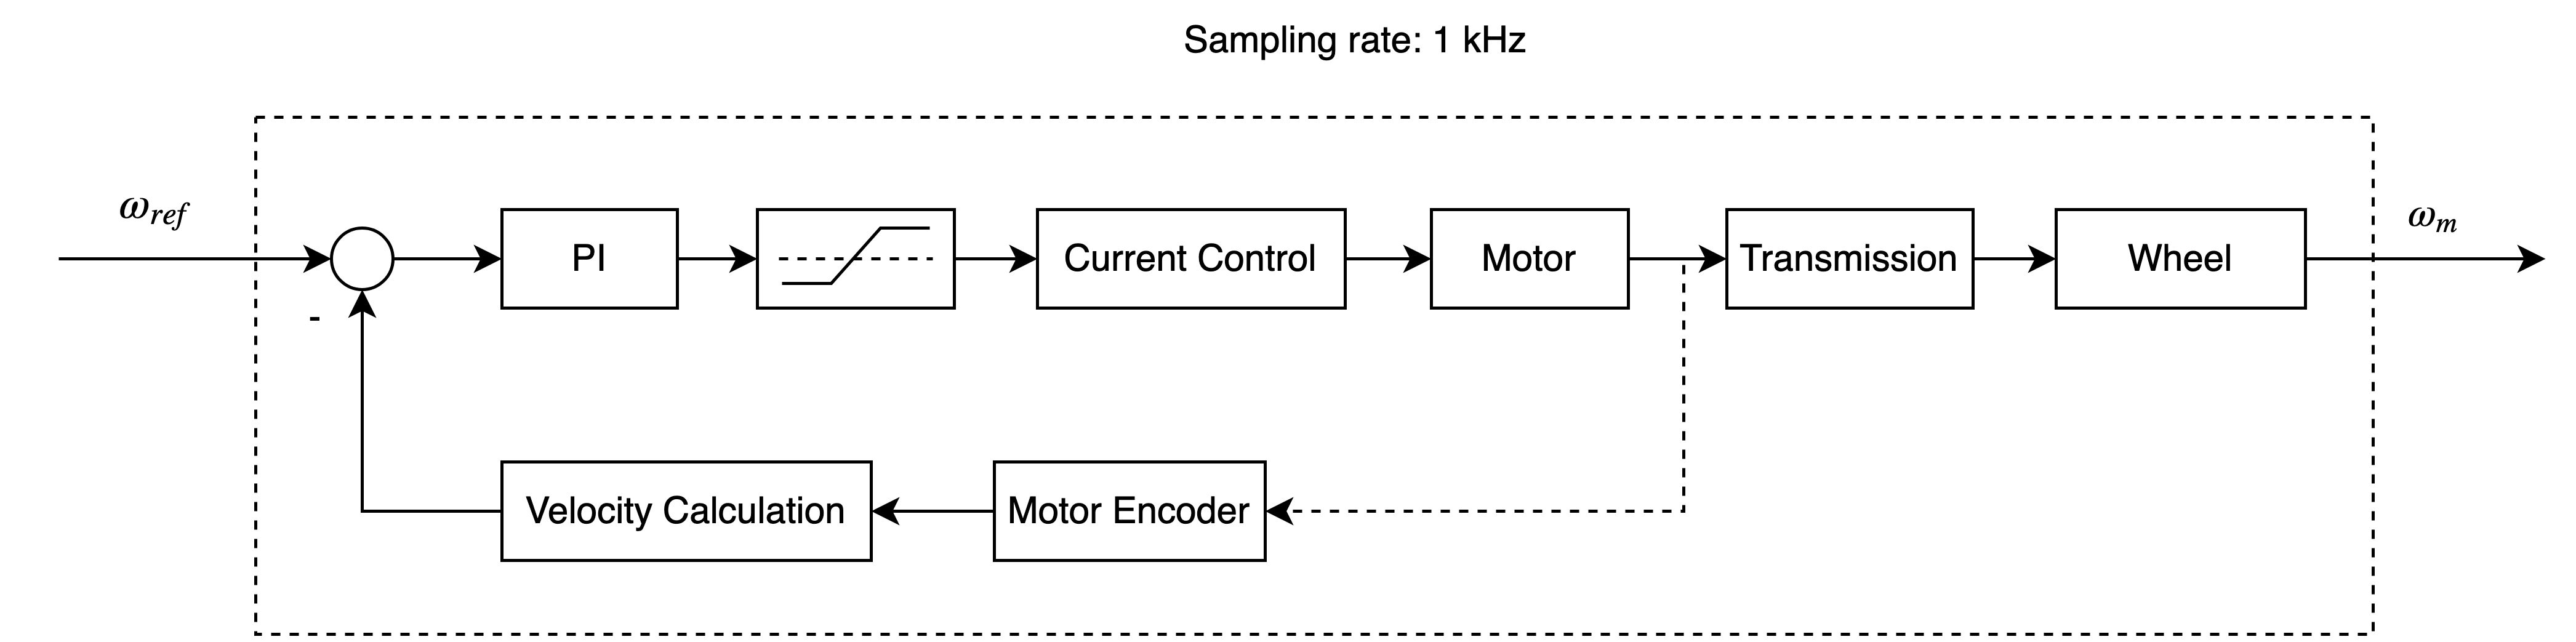
\includegraphics[width=\textwidth]{velocityControl}
	\caption{Block schema of the velocity control}	
	\label{fig:velocityControl}	
\end{figure}
\noindent 


\end{document}